\section{Prototype}
The overall functionalities for the project have been limited, due to time limitations and to focus on the scope of the project. In this project a prototype will therefore be made to show the main functionalities necessary to make an automated vehicle containing principles for lawn mowing.
In short, the final prototype includes a regulator, which will make it possible to follow a path from A to B. It is able to continue if the wireless connection is lost between the prototype and the GoT system for some duration. Furthermore it is able to plan a route within a given area and store these calculated data points locally, on the vehicle. The rough outline of the design is shown in \figref{fig:systemOverview1} to give an idea of the final prototype setup.

\begin{figure}[H]
	\centering
	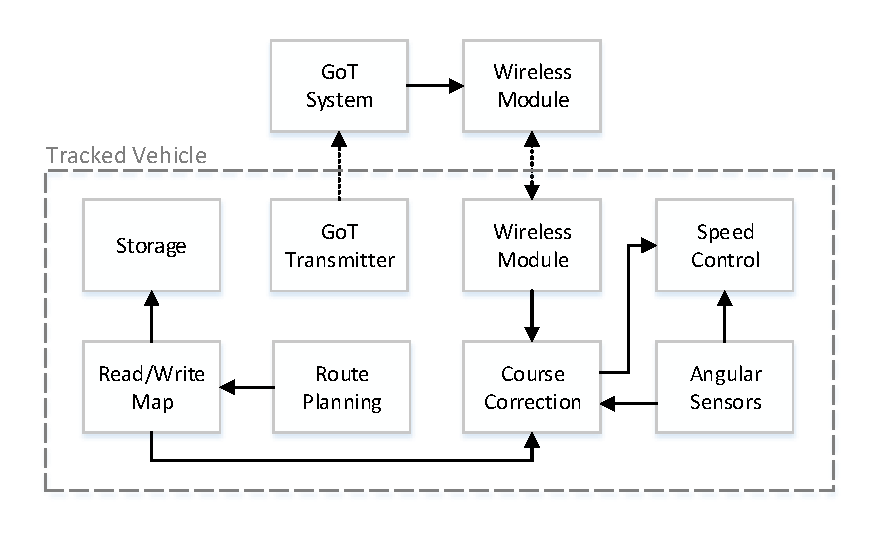
\includegraphics[scale=.9]{figures/systemOverview1}
	\caption{Overview of the system prototype}
	\label{fig:systemOverview1}
\end{figure}

The GoT system provides the vehicle with coordinates, which is utilized in course correction in combination with the map supplied from storage, to follow the route. In course correction lies also control between coordinates given by the GoT system and the storage, this is regulated through use of angular position and movement supplied by the angular sensors. The speed control gets an input from the course correction, the speed given is then held through regulation again using input from angular sensors, in this case specifically acceleration.

\section{Prototype Interfaces and Submodules}
Previously the rough prototype design is presented. To provide a more broad overview of the system, an exploded view of functionalities, their submodules and interfaces is presented in \figref{fig:systemOverview2}.

\begin{figure}[H]
	\centering
	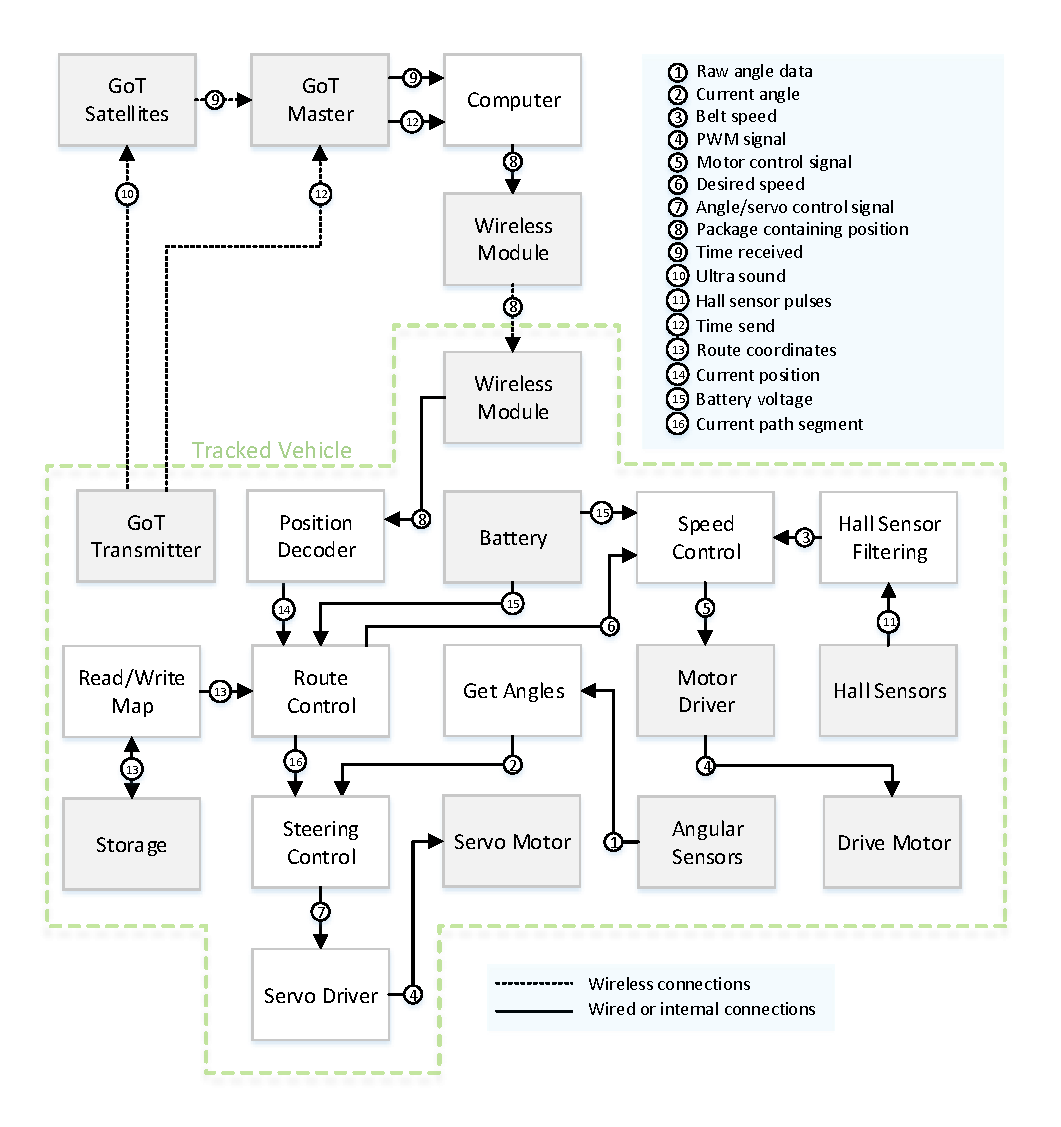
\includegraphics[scale=.9]{figures/systemOverview2}
	\caption{Expanded overview of the system prototype}
	\label{fig:systemOverview2}
\end{figure}

\subsection{Expansion of Modules}
- To Tom and Rasmus \newline
In this subsection, we have thought about making an explanation of the expansion of some of the different modules, form the first edition (see on \figref{fig:systemOverview1} and an a explanation of the new expanded modules functions in the prototype, seen in \figref{fig:systemOverview2}.  

\indent
%Apart from - \textit{Storage}, \textit{Read/Write Map} and \textit{Wireless Modules} - all the modules from the system prototype is expanded to more accurately describe the basis for the prototype. In the following a brief description of these expansions is presented.

\subsubsection{GoT System}
\indent
%\textit{GoT Satellites} \textit{GoT Master} \textit{GoT on Computer} \textit{Ultra Sound \& Radiolink}
%
%The GoT satellites is placed in the area in which the vehicle needs to operate. These satellites receives information from the vehicle. The time which the vehicles transmitter sends out bursts is received by the GoT master. Furthermore the time which the satellites receives the information send from the vehicles transmitter is transmitted to the GoT master. The GoT master then relays the information received from the vehicle directly to the 
%
%A number of GoT Satellites are placed in the corners of the area in which the vehicle is to operate. These Satellites receive ultra sound signal from the GoT device placed on the vehicle. The time in which each ultrasound signal is received is passed through a wireless connection from the satellites to the GoT master. The GoT master then pairs this information with the time the ultra sound signal was send from the vehicle which it receives via radio link from the GoT device on the vehicle. After collecting the information, the GoT master sends a calculated position and along with a time stamp to the computer handling GoT.

\subsubsection{Route Planning}
\textit{Route Planning} \textit{Edge Map}

\subsubsection{Speed Control}
\textit{Hall Sensors} \textit{Get Speed} \textit{Speed Control} \textit{Motor Driver} \textit{Drive Motor}

\subsubsection{Angular Sensors}
\textit{Get Angle} \textit{Angular Sensors}

\subsubsection{Course Correction}
\textit{Servo Motor} \textit{Course Correction}

\subsection{Interfaces}
- To Tom and Rasmus \newline
In the subsection an explanation of the different interfaces between the modules is made. We have thought about making it like a high layer interface, where we only explain what we need the different modules to give each other. Like one module needs to get the map edge, i.e. coordinates, but since it is this early in the report and it would be more overview by writing map edge rather than coordinates. But as you can see in \figref{fig:systemOverview2} the layers of information are different, one is raw angle data and another time send. Is this okay or should we change something else?
\indent
%The interfaces of the system is very important when designing each of the adjacent submodules. The existing interfaces as well as the ones presumed are also important in the process of analyzing the system capabilities width focus on requirements of the prototype. Width that in mind follows a brief review of the interfaces between each submodule.

\subsubsection{GoT System Interfaces}
\textit{Ultra sound} \textit{Time received} \textit{Position and time} \textit{Time send}

\subsubsection{Route Planning, Storage and Read/Write Map Interfaces}
\textit{Position and Time} \textit{Desired speed} \textit{Angle data} \textit{Angle/servo control signal}

\subsubsection{Speed Control Interfaces}
\textit{Map edge} \textit{Route}

\subsubsection{Angular Sensors Interfaces}
\textit{Raw angle data} \textit{Angle data}

\subsubsection{Course Correction Interfaces}
\textit{Desired speed} \textit{Angle data} \textit{PWM signal} \textit{Belt speed} \textit{Hall sensor pulses} \textit{Motor control signal}

%---------------------------------------------------------------------------------------------------------------------------\\
%REWRITE THIS SCRAMBLED VERSION OF THE ABOVE TWO SUBSECTIONS\todo{rewrite in the above section and delete these subsections}\\
%---------------------------------------------------------------------------------------------------------------------------

\subsubsection{GoT Satellites, Master and GoT Ultra Sound \& Radio Link}
\indent
%A number of GoT Satellites are placed in the corners of the area in which the vehicle is to operate. These Satellites receive ultra sound signal from the GoT device placed on the vehicle. The time in which each ultrasound signal is received is passed through a wireless connection from the satellites to the GoT master. The GoT master then pairs this information with the time the ultra sound signal was send from the vehicle which it receives via radio link from the GoT device on the vehicle. After collecting the information, the GoT master sends a calculated position and along with a time stamp to the computer handling GoT.

\subsubsection{Wireless Modules}
\indent
%The wireless modules serves the purpose of transmitting the calculated coordinates from the GoT system to the vehicle.

\subsubsection{Edge Map, Route Planning, Read/Write Map and Storage}
\indent
%The route planning functionality receives the hard coded edge positions from edge map. Using this information the route is then planned and saved in the storage through the read/write map functionality.

\subsubsection{Gyro, Accelerometer, Magnetometer, Speed Control and Course Correction}
\indent
%Gyro along with magnetometer is used for angular position of the vehicle. This is passed to the course correction through the get angle functionality. Here it is used as to correct the orientation of the vehicle on its path. The accelerometer also channels through the get angle functionality. The angular acceleration is then used for correction of the speed.

\subsubsection{Hall Sensor}
\indent
%The speed control also receives input from the hall sensors through the get speed functionality, where the inputs from the hall sensors are translated to speed of the vehicle's belts. This information is then used in speed control to regulate the speed.

\subsubsection{Servo Motor}
\indent
%The servo motor receives an angle/servo control signal from course correction. This angle equals a given amount of breaking on either of the two belts, which then through the differential gearing translate into steering and thus correction of the course of the vehicle.

\subsubsection{Motor Driver and Drive Motor}
\indent
%The drive motor takes a motor control signal from the motor driver provided by the speed control. The control signal from speed control is a PWM signal.